\chapter{Theoretical Framework}
\label{chap:theoretical-framework}

The following chapter will introduce the relevant theories and key concepts related to emotion recognition, such as speech-based and text-based models and technologies. 
This chapter will explain how vocal features and speech prosody can help to identify different emotions in spoken languages, using different AI tools and software. This study aims to compare accuracy and effectiveness of different approaches by conducting interviews and collecting data, which will be analyzed using a Python application. The elements of the Python application for analyzing the data from the interviews will be comprehensively explained in this chapter.

\section{Affective Computing}

 Affective computing was introduced by Professor Rosalind Picard in the mid-1990s to early 2000s \autocite{Tian2022}. By exploring the ways in which human emotions are recognized, understood and expressed through different forms of behaviors and communication, the domain of affective computing is a field that merges the principles of artificial intelligence with insights from social and behavioral science \autocite{Tian2022}.

\section{Natural Language Processing and Emotion Recognition}
The first English language lexical database was created in 1998 for Natural Language Processing (NLP) tasks, the term sentiment and emotional analysis came to practice in 2001 to predict the stock market, and in 2005 the first article was written on emotion and opinion detection from text \autocite{Kusal2023}. Concept-level sentiment analysis resources were publicly available in 2009. Word embedding is the term to represent words for NLP text analysis and was developed in 2013, the same year as neural network first was adopted in NLP tasks. The field had a massive upwelling when the transformers concept was published in 2017, followed by the evolution of BERT, a pretrained model that automated text analysis and classification in 2018 \autocite{Kusal2023}. 

Traditional approaches for sentiment analysis classification have been used since the past few decades, which rely on rule-based methods such as “bag of words” method to process text  \autocite{Kansara2020}. The method represents text based on word frequency without consideration of word order. It can identify sentence structure, negation, emphasis, subjectivity and irony. Recent models leverage deep learning algorithms that process raw text by first cleaning and pre-processing it, including punctation, stop words and markups, as well as applying stemming (the process of reducing words to their root form by removing prefixes or suffixes to simplify text analysis in NLP). 

Deep learning applicate artificial neural networks (ANN) to learn tasks using multiple layers of network. In traditional models only one or two layers could be used, but in deep learning much more learning power of artificial neural networks is exploited \autocite{Zhang2018}. Studies have shown consistently higher accuracy for sentiment analysis using deep learning algorithms compared to traditional machine learning algorithms \autocite{Kansara2020}.


\section{Speech-Based Emotion Recognition}

Studies about speech-based emotion recognition (SER) have been ongoing since 1978 \autocite{LGENSNMEZ2024}. SER identifies how something is being said without the context of the words spoken. These systems are used in many different areas, most often in areas of interactions between humans and machines (Zhang, 2025). 
A typical SER system contains of three components: signal preprocessing, feature extraction, and classification \autocite{Sahoo2023}.

Although there is a wide range of SER-algorithms, with some approaches using more complex setups that involve Convolutional Neural Networks (CNN) based SER algorithms among others \autocite{Ri2023}, the process of a SER algorithm could look like figure \ref{fig:stages-SER}, involving several steps as feature extraction, selection and classification.


\begin{figure}[ht]
    \centering
    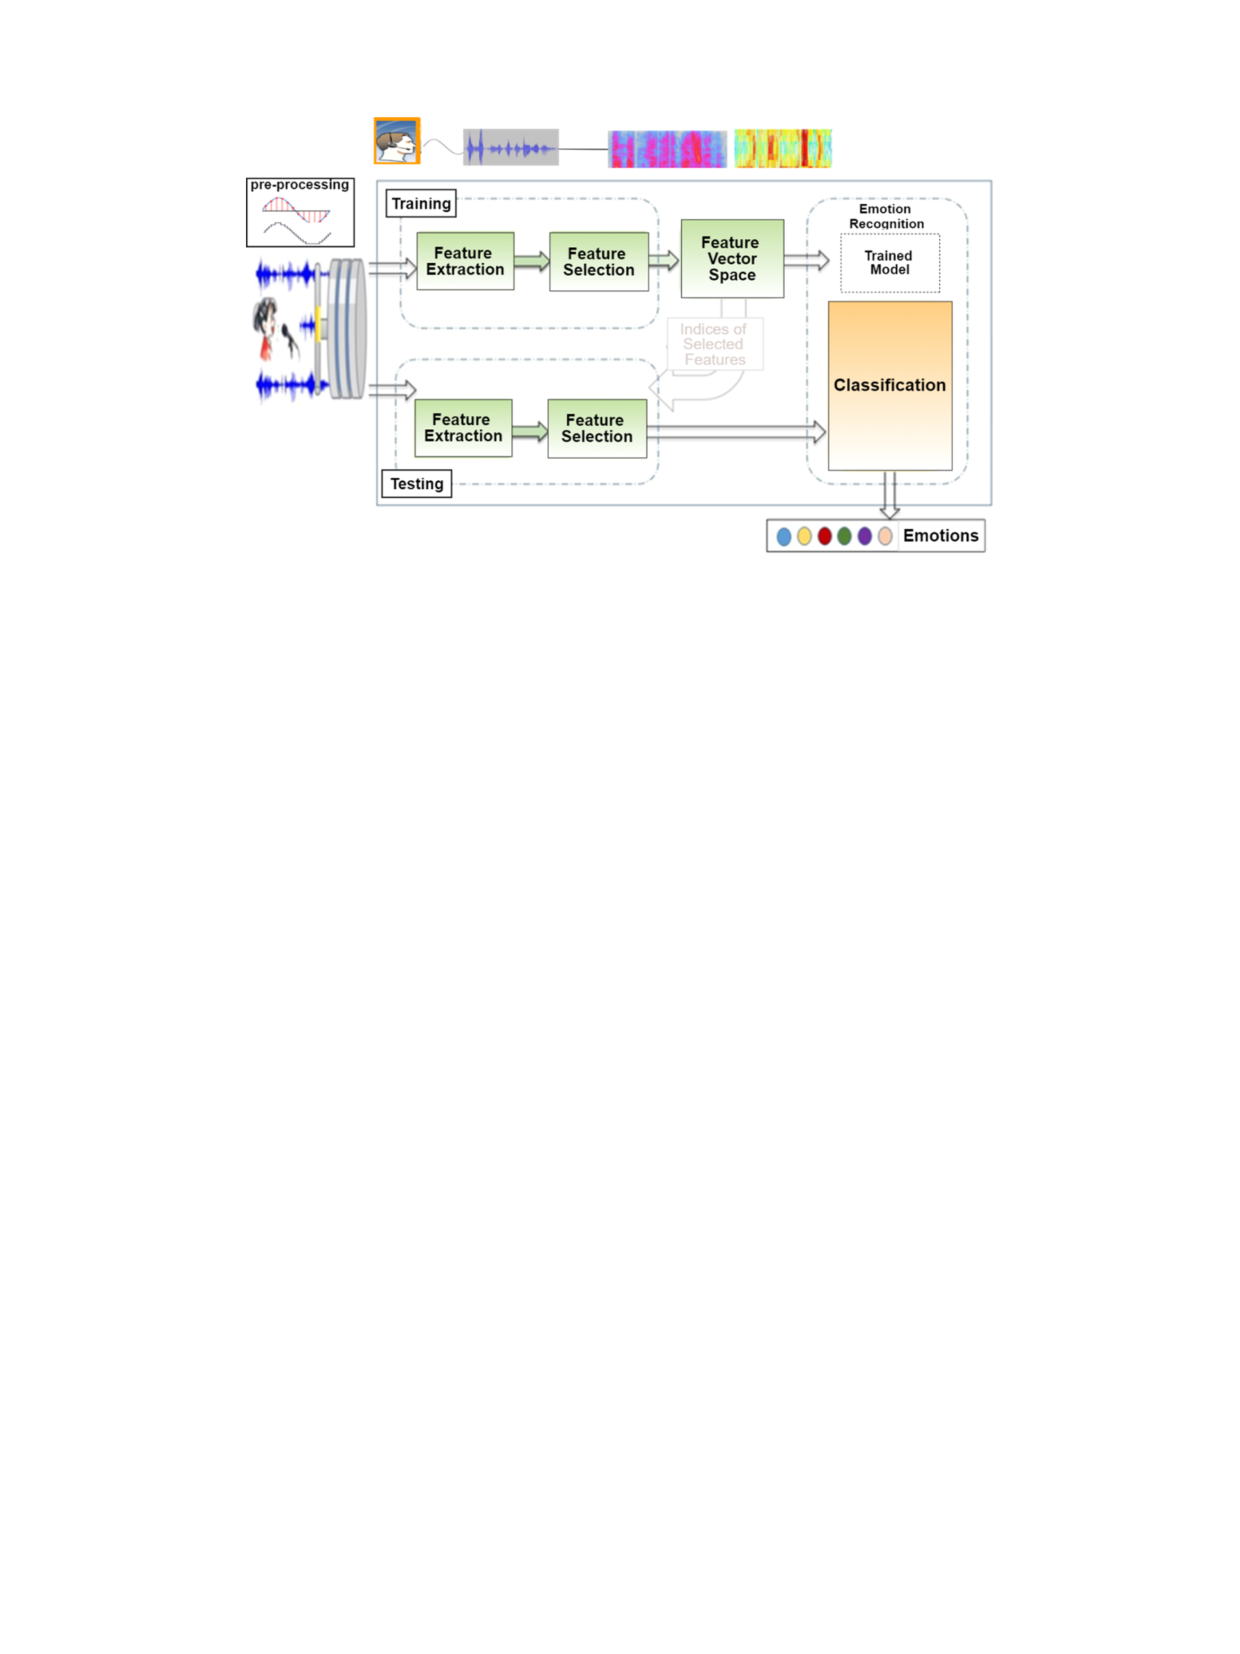
\includegraphics[width=10cm]{png/theoretical/ser-diagram.pdf}
    \caption{\textit{An overview of the stages in SER to analyze speech data for emotion detection} \autocite{LGENSNMEZ2024}}
    \label{fig:stages-SER}
\end{figure}
 
While emotions can be recognized via many channels such as speech, facial expressions and text, speech signals are rapid and natural which makes vocal audio fitting for emotion recognition. According to \textcite{LGENSNMEZ2024} there are several key benefits with SER, such as a limited amount of hardware needed for the capturing the vocal data which simplifies the process of the vocal data collection. Another benefit is that vocal data being less demanding in terms of storage, compared to video footage for example, and participants in SER experiments may feel more comfortable with vocal analysis than face analysis in terms of confidentiality, resulting in datasets reflecting real emotions more accurately.

\subsection{Hume AI }

Hume is a technology company dedicated to advancing the field of emotion recognition. Having conducted extensive psychology studies to explore human emotions and the way these emotions are expressed, Hume AI has used the research to develop advanced machine learning models \autocite{HumeAi-aboutScience} as well as using deep learning for the research and development \autocite{Brooks2023}.

The official website of Hume AI outlines several influences on their emotional mapping. Drawing influence from key figures such as David Hume, Charles Darwin and Paul Ekman, Hume AI’s research is grounded in these foundational theories of emotions. Paul Ekman’s “The Basic 6” is mentioned \autocite{HumeAI-AboutHume} and remains relevant throughout this research. 

One of the measurements used to recognize emotions in vocals with Hume AI in this research is speech prosody. 

Speech prosody gives crucial insights into a speaker’s purpose in their communication. Particular emotions and the intensity of those emotions are indicated with intonation, rhythm and pitch of the speaking voice \autocites{Thompson2004}{Tomasello2022}. It simply refers to the patterns and tone in the speech that are not related to the actual words being spoken \autocite{Cowen2019}.

Happiness and sadness show the opposite characteristics of each other, where happiness is linked to quicker tempo and higher pitch while sadness has the opposite, a slower tempo and lower pitch. The clear difference between the characteristics serves as the difference in the speech prosody of the two emotions \autocite{Thompson2004}. 

In figure \ref{fig:hume-ai-speech-prosody}, a visual presentation of Hume AI’s speech prosody model is visible \autocite{HumeAIProsody}. Emotions are clustered with other similar emotions, one example being amusement and joy, or distress and anxiety.

\begin{figure}[ht]
    \centering
    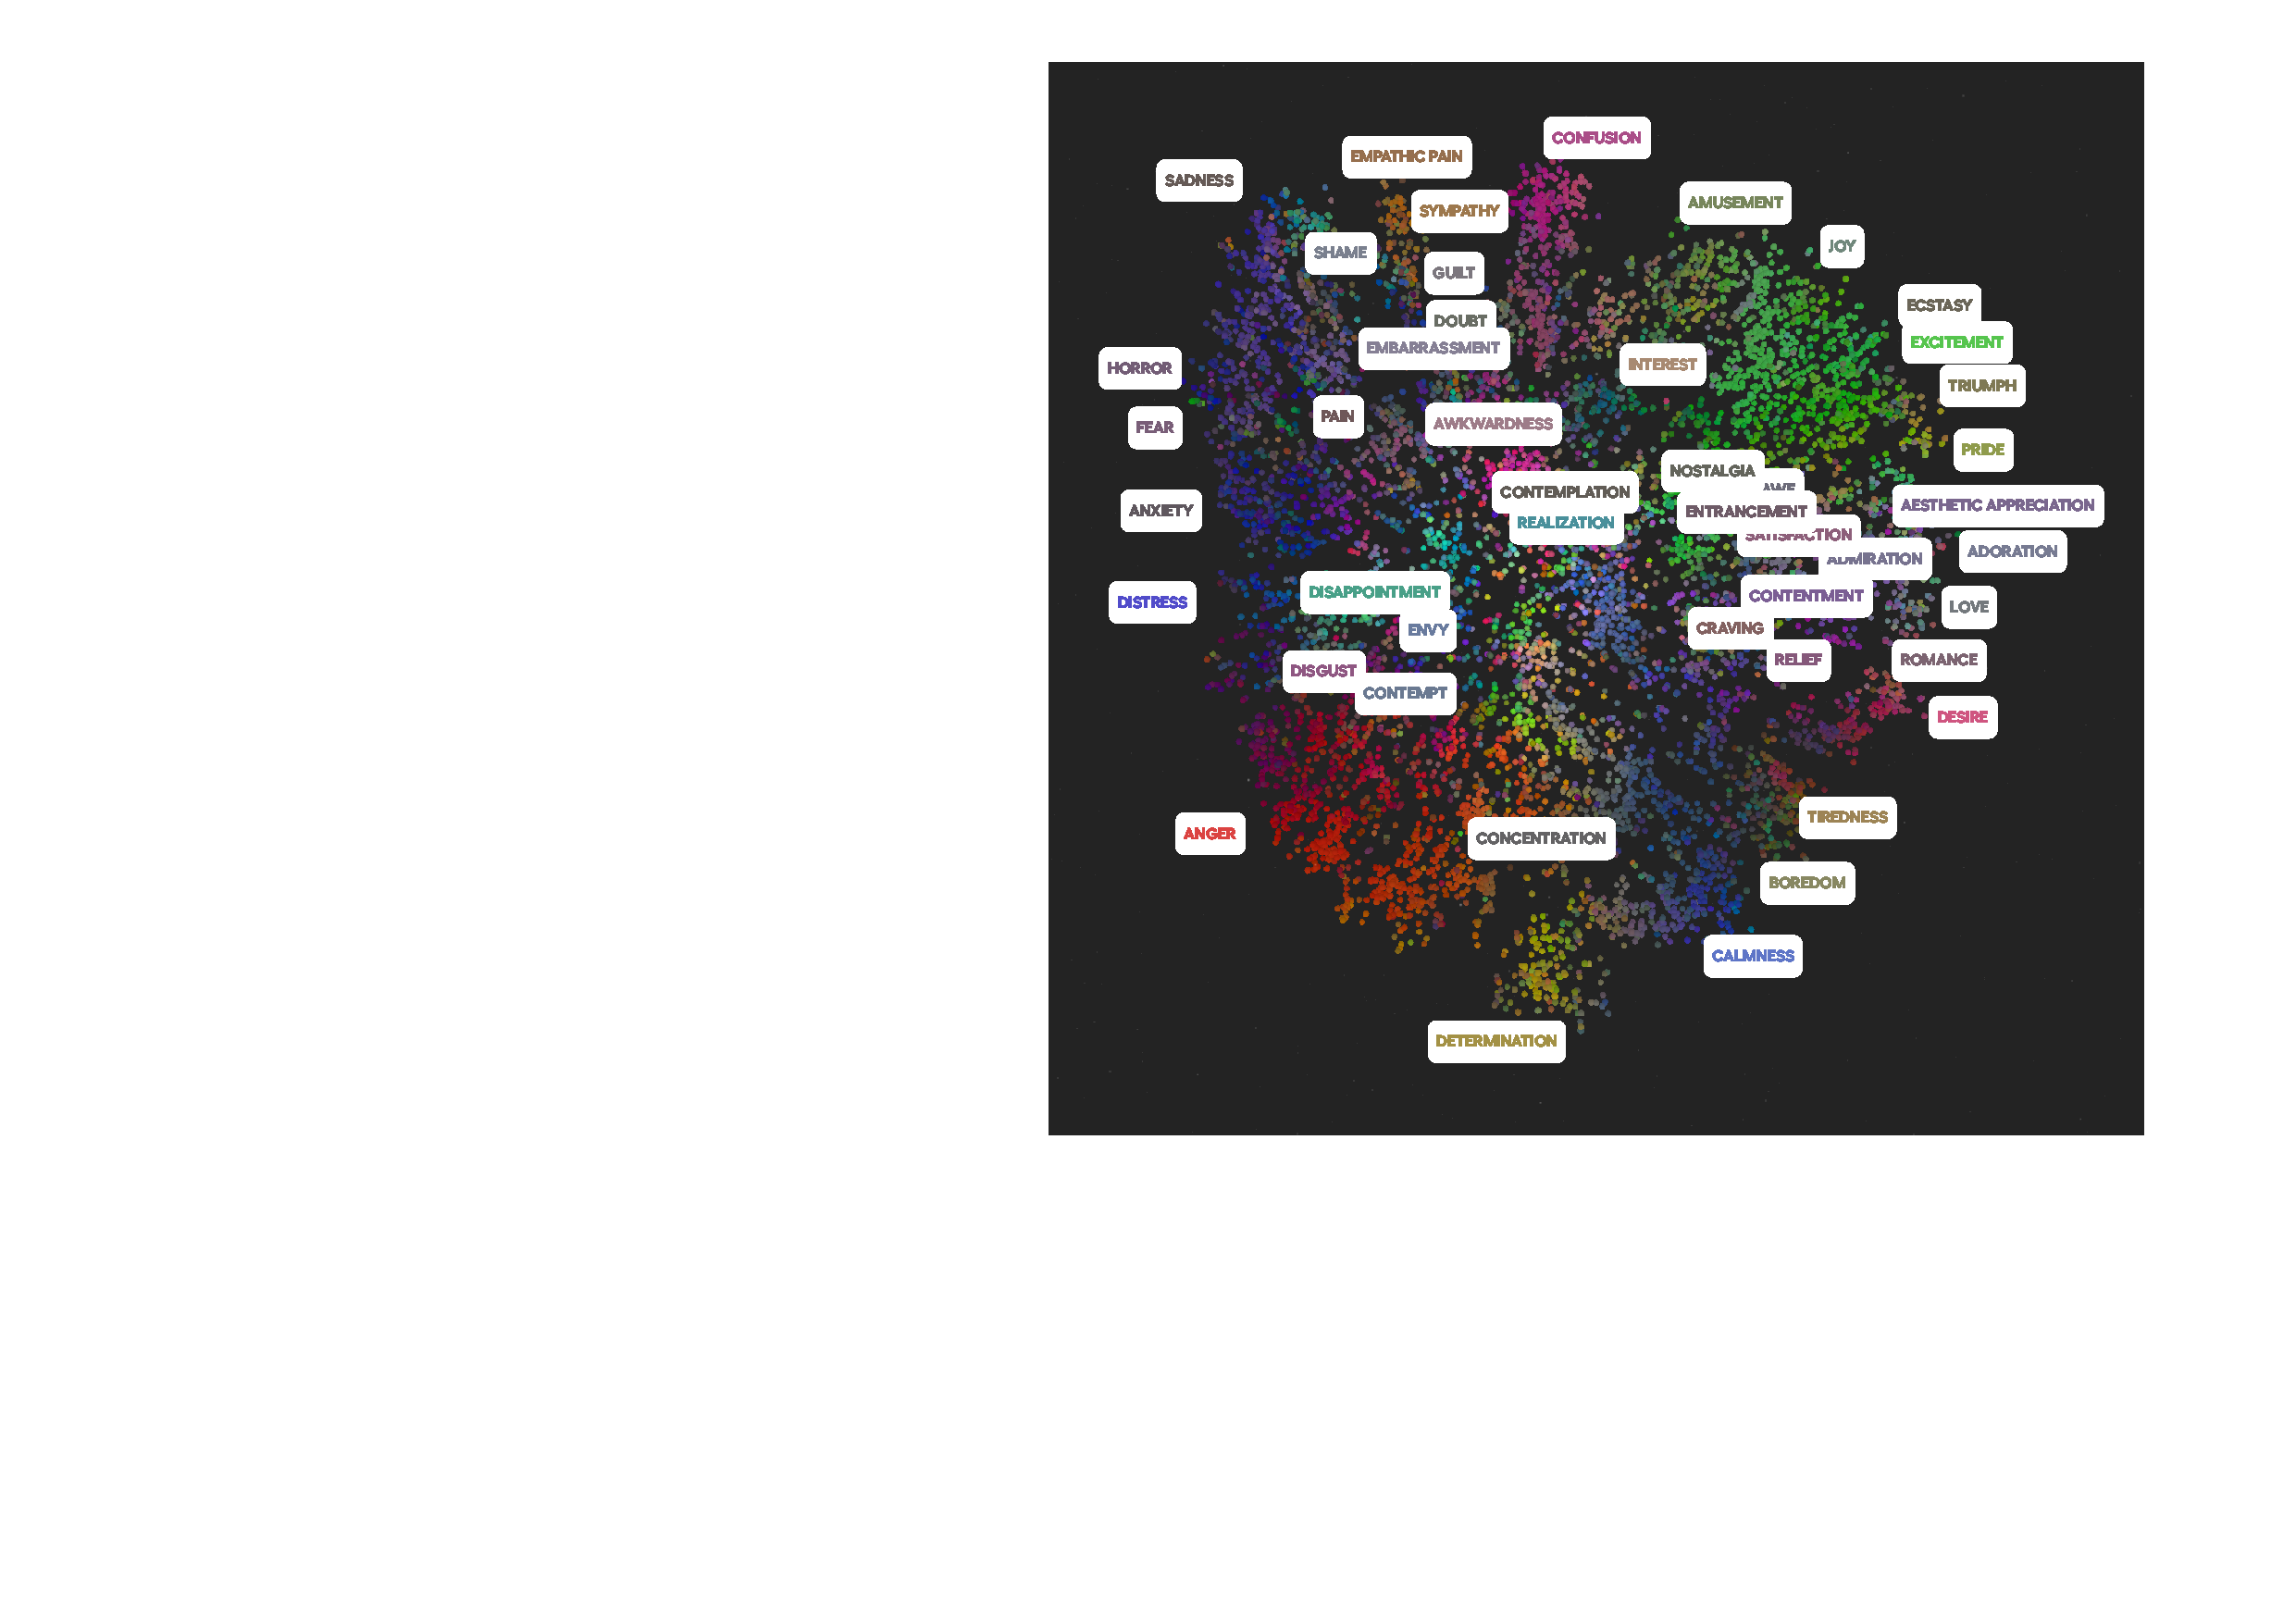
\includegraphics[width=10cm]{png/theoretical/hume-prosody.pdf}
    \caption{\textit{Visual representation of Hume AI’s speech prosody model} \autocite{HumeAIProsody}}
    \label{fig:hume-ai-speech-prosody}
\end{figure}

To ensure a broader range of emotion recognition with a more comprehensive analysis of human voices in this research, speech prosody is used in combination with another measurement, vocal bursts.

Vocal bursts play a key role in social communication between humans. They are short emotional sounds which occur naturally, some examples being laughs, sighs or cries \autocite{Brooks2023}.

Vocal burst and voice have received less attention in the fields of machine learning and affective computing due to more focus being held on facial expressions. Even if speech prosody has been studied more extensively, there has been newer research showing that vocal bursts convey more than ten different emotions with consistency, being mostly consistent across different cultures as well \autocite{Baird2022}.

Figure \ref{fig:hume-ai-vocal-burst} shows Hume AI’s mapping of non-verbal communication, vocal bursts \autocite{HumeAIVocalExpression}. Emotions are shown and as well as in Hume AI’s speech prosody model, the emotions are clustered indicating some emotions are more associated with each other.

\begin{figure}[ht]
    \centering
    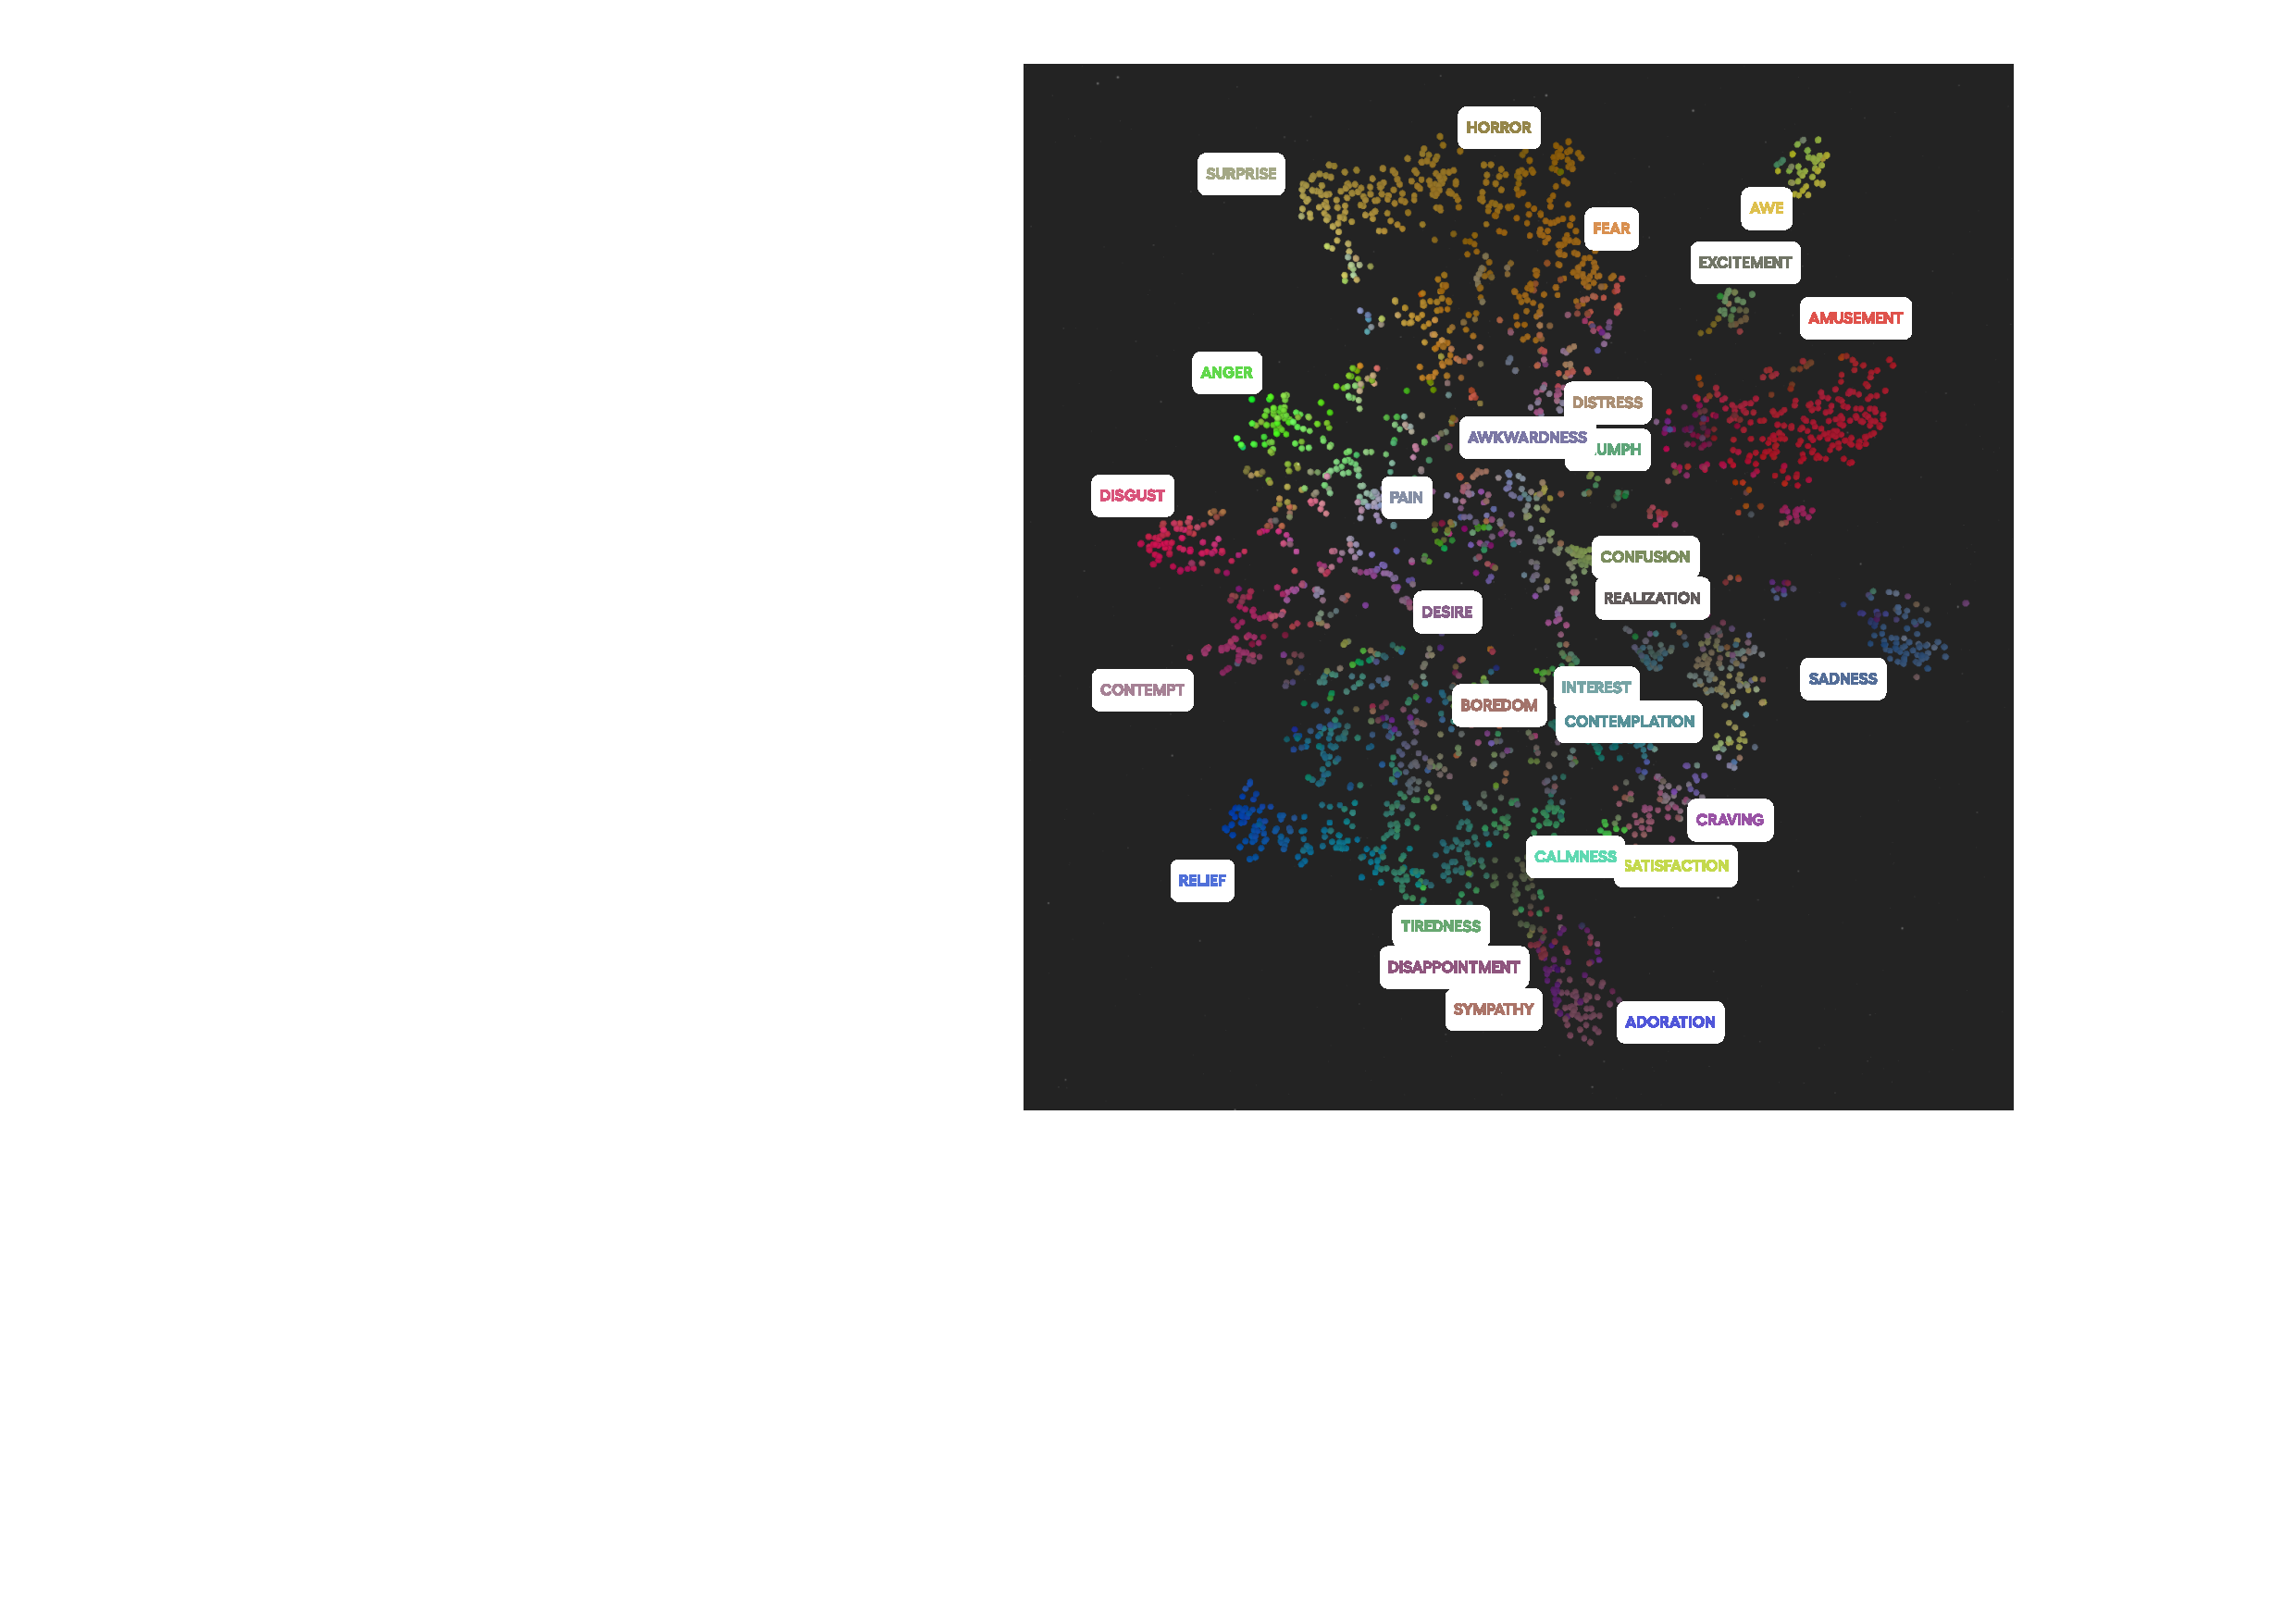
\includegraphics[width=10cm]{png/theoretical/hume-vocal.pdf}
    \caption{\textit{Visual representation of Hume AI’s vocal burst model} \autocite{HumeAIVocalExpression}}
    \label{fig:hume-ai-vocal-burst}
\end{figure}

While there are other tools for emotion recognition, Hume AI is among the few that are specifically designed for Voice AI while being able to recognize emotions through specifically speech prosody and vocal burst with no need to finetune it yourself. 
Using models needing finetuning would not fit the scope of this thesis given the limited timeframe, and while there are other models, like OpenAI whisper, which is an extensively trained model on hundreds of thousands of hours on data, their main focus leans toward transcribing speech \autocite{OpenAI2022}. This ultimately led to the decision to use Hume AI.

\subsection{Praat Parselmouth}

In the field of software for linguistic analysis, Praat is a well-established tool to analyze different elements in speech. Being able to estimate elements such as fundamental frequency and intensity among others, Praat holds a broad spectrum of algorithms in acoustics, being a successful tool for analyzing acoustics \autocite{Jadoul2024}.

Designed to provide efficient access to the core functionalities of Praat in Python for programmers, Parselmouth is an open-source Python library \autocite{Jadoul2018}.

Python is widely used for data analysis, but it had been noted that there were challenges with analyzing acoustics in Praat, this due to the functionality often being missing or scattered across multiple incompatible libraries.

Parselmouth streamlines and optimizes workflows in a single programming environment by enabling a deeper integration of the capabilities of Praat in combination with other libraries \autocite{Jadoul2024}. Not designed to replace Praat, but rather a way to enable users to access the functionality of Praat directly in Python, there some main objectives in Parselmouth according to \textcite{Jadoul2018}.
One objective is to enable users already experienced with Praat to effectively incorporate its functionality with Python’s scientific tools, being tools that are not obtainable in Praat.
Providing Python users with the ability to utilize the functionality of Praat, even if they are not experienced users of it, is also an important aspect, as well as enhancing the optimal aspect of workflow for users preferring to conduct their work within a single programming language.
 
The benefits of Parselmouth both in terms of the usage for completing this thesis and overall, are it being open source and compatible with Python as Python is widely utilized and backed by a vast community of researchers and engineers, among others. Parselmouth integrates the different strengths of different approaches to provide a library following the principles of Python and behaving consistently with other well-known Python libraries.

Parselmouth directly utilizes the official C/C++ source code of Praat instead of having to reconstruct its algorithms. This simplifies the process since it guarantees full consistency with Praat without the requirement of learning its scripting language \autocite{Jadoul2018}.

There are other similar tools that essentially could accomplish the same task, like Librosa although it is more tailored for both audio and music analysis. It does have feature extraction \autocite{Babu2021}, but the decision on which software to use for linguistic analyzation still falls on Praat Parselmouth due to it being more fitting for the purpose of this thesis.

\section{Text-Based Emotion Recognition}
In the field of NLP, the comprehension of the context behind words in text-form has gone from only being able to determine the tone in text to actually identifying the emotions behind them \autocite{Esfahani2024}, recognizing these capabilities has valuable practical applications in enhancing different domains within human-computer interaction \autocite{Shelke2022}. 
Text-based systems rely strongly on lexical cues, and research shows different types of words carries different levels of intensity \autocite{Chauhan2024}. This highlights both a strength and a limitation of text-based emotion recognition, as emotional sentiment may go undetected unless it is verbalized, since emotions may not necessarily be expressed through text \autocite{Soleymani2017}.

Text-based emotion detection relies on four main approaches, according to \textcite{Kusal2023}.
The first approach is keyword-based, which matches words in a text with predefined emotion keywords from resources like WordNet, adjusting for intensity and negation. The second approach is rule-based, and this approach uses linguistic rules and probabilistic affinity to classify emotions after preprocessing. The third is machine learning-based which applies supervised or unsupervised models to classify emotions, extracting key features from preprocessed text. The fourth and last approach is deep learning-based and it utilizes neural networks to learn complex patterns from tokenized and embedded text data for emotion classification.

Machine learning classifiers are significantly used in text-based classification, since they use labeled datasets and are therefore data driven. Machine learning models are trained on large number of datasets and learn from experience, with classifiers that contain labels for input and desired output. Transformer-based models, such as BERT, are based on machine learning models which are trained on vast amounts of data and can be fined-tuned for specific tasks. BERT is a deep learning model based on attention processing. It gains a thorough text-understanding through considering left and right contexts equally. The model solves NLP issues and is used to train general language models on large datasets \autocite{Kusal2024}.

\subsection{NLP Cloud}

There are limited publicly available APIs for text-based emotion detection (TBED). The decision to use NLP Cloud for this study consists of several reasons as following. Compared to other available TBED APIs that do not require pre-training, NLP Cloud has comprehensive documentation for both API and the models that it is based on. The company has support as well as information about Data Privacy and Security \autocite{NLPCloud}, which also other APIs for TBED has. For example, Vern AI (AI, u.d.) provides customer support but has very limited information about the API or documentation that is easily accessible. TwinWord \autocite{TwinWord} was another choice, also providing contact support and privacy information, but was deficient in comprehensive documentation and limited information about the API. 
In addition to what is mentioned above for factors of why this model was chosen, NLP Cloud have established customers like Zoom, and collaborations with Nvidia, which underscores the credibility and relevance of the company. They provide information about what models they use for their API which can be downloaded and fine-tuned if desired. In contrast to the other APIs, NLP Cloud provide APIs for Speech-to-Text transcription, and they have an emotional analysis model supporting Swedish Language. Therefore, no translation is required beforehand, enabling direct processing of Swedish language preserving emotional details which may otherwise have been lost in translation, being another reason as to why the choice landed on NLP Cloud. Their speech-to-text API is based on OpenAI’s Whisper model \autocite{NLPCloud}. OpenAI provides a research report on the model, which is a speech recognition system designed to process and transcribe audio with robustness and generalization. Contrasting traditional models that heavily rely on unsupervised pre-training or dataset-specific fine-tuning, Whisper leverages large-scale weakly supervised training from over 600,000 hours of multilingual audio data. This includes 96 languages beyond English. Whisper handles several tasks, for instance speech recognition, language identification, and translation \autocite{Radford2022}. 

For sentiment and emotion analysis, NLP Cloud provides several options. Two of them are equally researched with relatively comparable results. DistilBERT Base Uncased Emotion is one option, with studies on DistilBERT, and Transformer-model which require finetuning and require less computational resources than traditional BERT (Bidirectional Encoder Representations from Transformers) models \autocite{NLPCloud}. The model was developed by Google and released in 2018 \autocite {Qazi2025}. BERT has challenges regarding fixed input length and computational complexity, reasons that led to DistilBERT’s development in October 2019. This pre-trained model uses technology that accomplishes to reduce a BERT model by 40\% while preserving 97\% of language understanding capabilities 60\% faster. The model accuracy for sentiment analysis ranges from 95.7\% to 96.6\% on Yelp Open Dataset, which has been demonstrated as a valuable resource of sentiment-labeled review-data \autocite{Areshey2024}. NLP Cloud provides a pre-fine-tuned version of DistilBERT. However, it does not support Swedish language, and translation beforehand is necessary for this study. A fine-tuned version of Llama 3 is an option on NLP Cloud that support several languages including Swedish \autocite{NLPCloud}. Opposed as to DistilBERT, some studies on emotion detection have been conducted on Llama 3. Both models have predominantly been evaluated for sentiment analysis. Emotion identification using Llama 3 showed an F1 score of 0.48 as average for all tested emotions: anger, joy, sadness, surprise, fear, and love \autocite{Zhang2024}. A fine-tuned version of Llama 3 was tested for sentiment analysis, which resulted in an accuracy increase from 0.333 to 0.923 and F1 score from 0.50 to 0.91. The authors of this study imply that these results are superior performance against other models that are included for comparison, including DistilBERT \autocite{Kumar2024}. In a text classification study, mainly examines speed performance, DistilBERT had an accuracy between 0.94-0.96 for the Amazon Alexa Reviews dataset but 0.35-0.41 for the Brexit Blog Corpus dataset \autocite{SilvaBarbon2022}. As for many models for emotion recognition mentioned in this report, the dataset affects the results heavily. 

Regarding multiple language performance, a study examined Llama 3 vs. State-of-the-Art Large Language Models on their ability to detect fake news. Two datasets were tested, one Romanian and one English. Their proposed Llama 3 model accomplished higher precision and accuracy across several metrics in fake news detection. For the English dataset, the fine-tuned Llama 3 model had lower accuracy compared to ChatGPT 4 and Gemini. Yet, it outperformed these models for the Romanian dataset, which is noteworthy considering both Romanian and Swedish are underrepresented languages in fields of LLM’s and NLP relative to English for example. The study also explored their fine-tuned Llama model compared to its base version. The fine-tuned model outperformed earlier models in distinguishing nuanced categories, particularly for the Romanian dataset where it achieved a remarkably high accuracy of 68\% in one category \autocite{Repede2024}.

Comparing these two alternatives for text-based emotion detection in Swedish, the fine-tuned Llama 3 model shows promise as the most suitable choice. Although the exact fine-tuned version of the model available on NLP Cloud has not been publicly researched, its built-in compatibility with Swedish, combined with research on a Romanian dataset, makes it a stronger candidate than DistilBERT. Both models have achieved high accuracy for TBED. Nevertheless, given this study is aimed to focus on emotion recognition models for Swedish speech, the Llama model without need for prior translation is a more valuable choice.

 

\section{Vocal Markers}
\label{sec:vocal-markers}

Vocal features have a significant role in distinguishing emotion through speech. It has been demonstrated that a listener accurately can recognize different emotions based on vocal cues, suggesting that emotional vocal expression has different patterns \autocite{Banse1996}. Acoustic variables that are involved in signalling emotions vocally include the fundamental frequency (pitch), vocal energy (intensity, loudness), the location of frequency formants (F1, F2, F3) which is associated with how articulation is perceived, and speech tempo. 
High arousal states include increased pitch and intensity, are related to positive emotion states as happiness/joy. These features indicate the same in Swedish \autocite{Ekberg2023}, where acoustic markers for five different emotions (anger, happiness, fear, sadness, surprise) were studied on fourteen acted sentences, each sentence articulated expressed with each emotion. Happiness presented highest fundamental frequency, increased loudness (intensity) and second highest harmony-noise-ratio (HNR). These results describe the largest pitch SD (6.25) for happiness, implying acoustic variability. 
Similar patterns are presented in a review on 108 studies \autocite{Kamilolu2020}, including twenty-six that researched acoustic features on positive emotions. Pitch, loudness, and formant features revealed the strongest indicators of positive emotions when compared with neutral vocalizations. The review suggests candidates as HNR indicating happiness as well but explain that clear conclusions cannot be composed due to limited empirical evidence. 
Anger shares increased pitch and vocal energy with joy \autocite{Banse1996}. The Swedish study indicates this pattern as well, although anger is not captured by frequency features separately but by amplitude cues as HNR and intensity \autocite{Ekberg2023}. HNR exhibited lower values than for happiness and fear, but higher than sadness and surprise. 
Sadness is predicted by lower intensity and pitch with slower speech rate, aligning with results on the Swedish language \autocites{Ekberg2023}{Scherer2003}. 
Vocalised fear is associated with panic in \autocite{Banse1996}, where pitch and frequency formants are heightened with increased rate of articulation. The Swedish report does not describe fear aligned with panic, although the opposite is not mentioned. The results showed second highest pitch, third highest loudness, and top HNR value. Frequency related jitter distinguished fear with the lowest value of the emotions. 
Jitter alongside amplitude associated shimmer characterised surprise in the Swedish results, with lower loudness and pitch than anger and happiness. Surprise is not included with listed values in the other studies referred to in this subsection. 

The results from the Swedish study \autocite{Ekberg2023} on emotional acoustic features are presented in Figure \ref{fig:compare-acoustic-parameters} with mean and standard deviation values for the five emotions. Other studies mentioned \autocites{Banse1996}{Kamilolu2020}{Scherer2003} and additionally Figure \ref{fig:acoustic-variations} \autocite{Khalil2019} demonstrate similar vocal expression patterns, but are mainly studied on English. 
Therefore, the results from the research on Swedish speech will serve as our reference when categorising emotions based on vocal markers in this study. 

 Figure \ref{fig:compare-acoustic-parameters} \autocite{Ekberg2023} shows a table of comparisons with certain parameters of vocal markers measured for five different emotions in the Swedish language and some explanations for the different parameters. This is used in this thesis as a comparison for the vocal markers collected from the interview data in the conducted experiment, although this thesis does not use all acoustic features to measure emotions.
 
\begin{figure}[H]
    \centering
    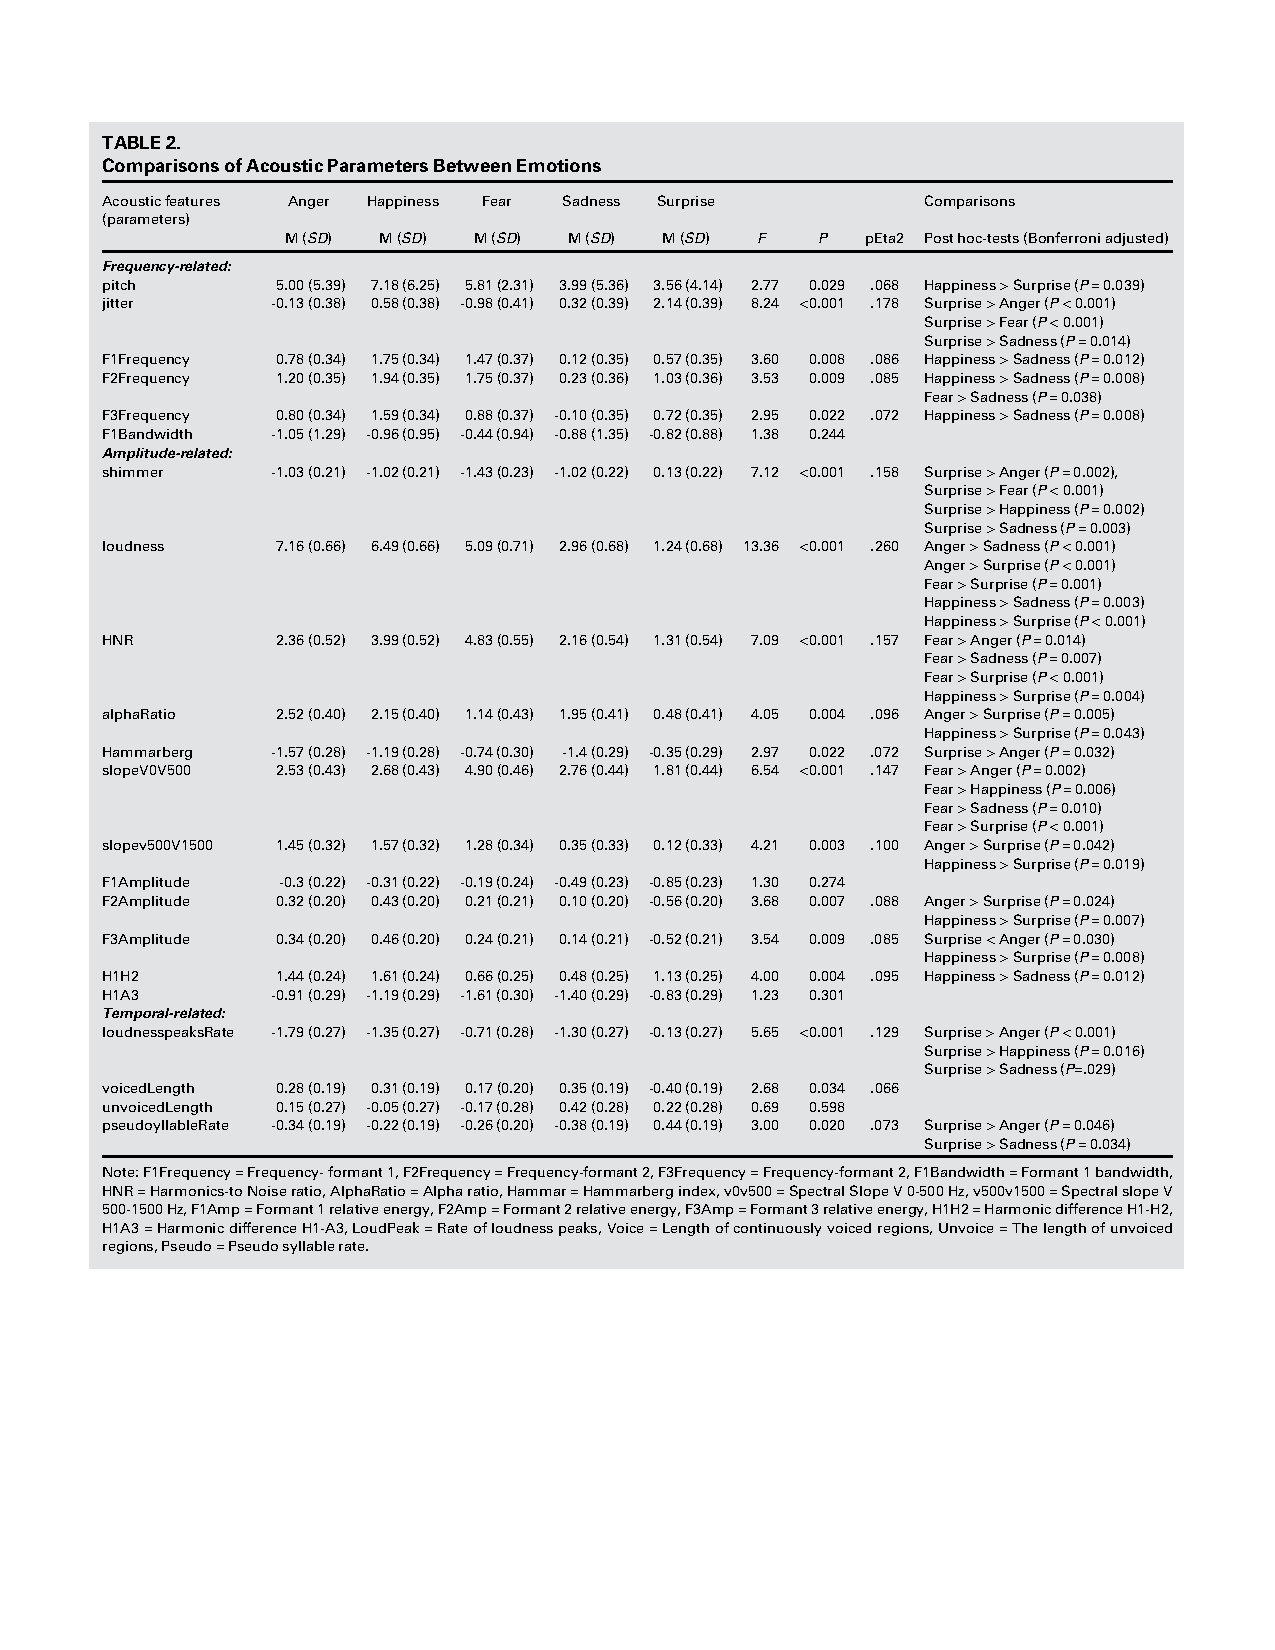
\includegraphics[width=10cm]{png/theoretical/table-acoustic.pdf}
    \caption{\textit{Table comparing acoustic parameters between emotions} \autocite{Ekberg2023}}
    \label{fig:compare-acoustic-parameters}
\end{figure}

The mean loudness divergencies between different emotions is shown in table \ref{fig:compare-acoustic-parameters} come with a very small standard deviation (e.g. $\sigma$ = 0.66 for anger mean = 7.16, happiness mean = 6.49). Contrasting, pitch differentiates between 2-6 $\sigma$. 
This suggests that loudness varies far less reliably than pitch across anger, happiness and fear. According to \textcite{Banse1996} is the fundamental frequency (pitch) the most studied and perceptually prominent feature. Happiness is one of the emotions that can be identified from pitch, yet both \textcites{Banse1996}{Ekberg2023} shows this positive emotion a wide overall acoustic spread. 
Figure \ref{fig:acoustic-variations} shows a table of variations in different emotions measuring the acoustic parameters pitch, intensity, speaking rate and voice quality which are often used to identify emotions \autocite{Khalil2019}. Additionally, Figure~\ref{fig:acoustic-variations} displays a wider variety of more specific acoustic features, figure 3.5 provides a foundational understanding of different acoustic features connected to the different emotions.

\begin{figure}[H]
    \centering
    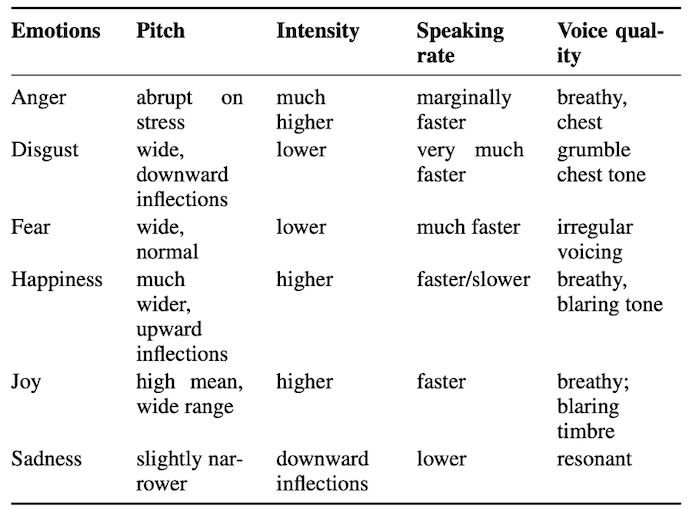
\includegraphics[width=8cm]{png/Figure8-AcousticVariations.png}
    \caption{\textit{Acoustic variations in different emotions} \autocite{Khalil2019}.}
    \label{fig:acoustic-variations}
\end{figure}

\section{The Experiment}

An experiment was be conducted and will consist of short voluntary interviews. These interviews were recorded for data collection and used to extract emotions with a Python application and analysed with a speech-based and text-based AI model.

\subsection{Python Application}

The Python application serves as the central system for processing and analyzing emotions in speech and will integrate several tools and frameworks to extract emotions. The overall structure is illustrated in Figure~\ref{fig:tf-python-app}.

The steps for the process consist of:

\begin{enumerate}
    \item Audio recording
    \item Feature extraction
\end{enumerate}

\begin{itemize}
    \item Prosody and vocal bursts will be analyzed with Hume AI to detect emotional cues from pitch, intonation and vocal bursts using Hume AI’s models.
    \item Extracting vocal features such as jitter, shimmer and frequency with Praat Parselmouth.
    \item Convert speech to text and analyze emotions in text with NLP Cloud.
\end{itemize}

\begin{figure}[H]
    \centering
    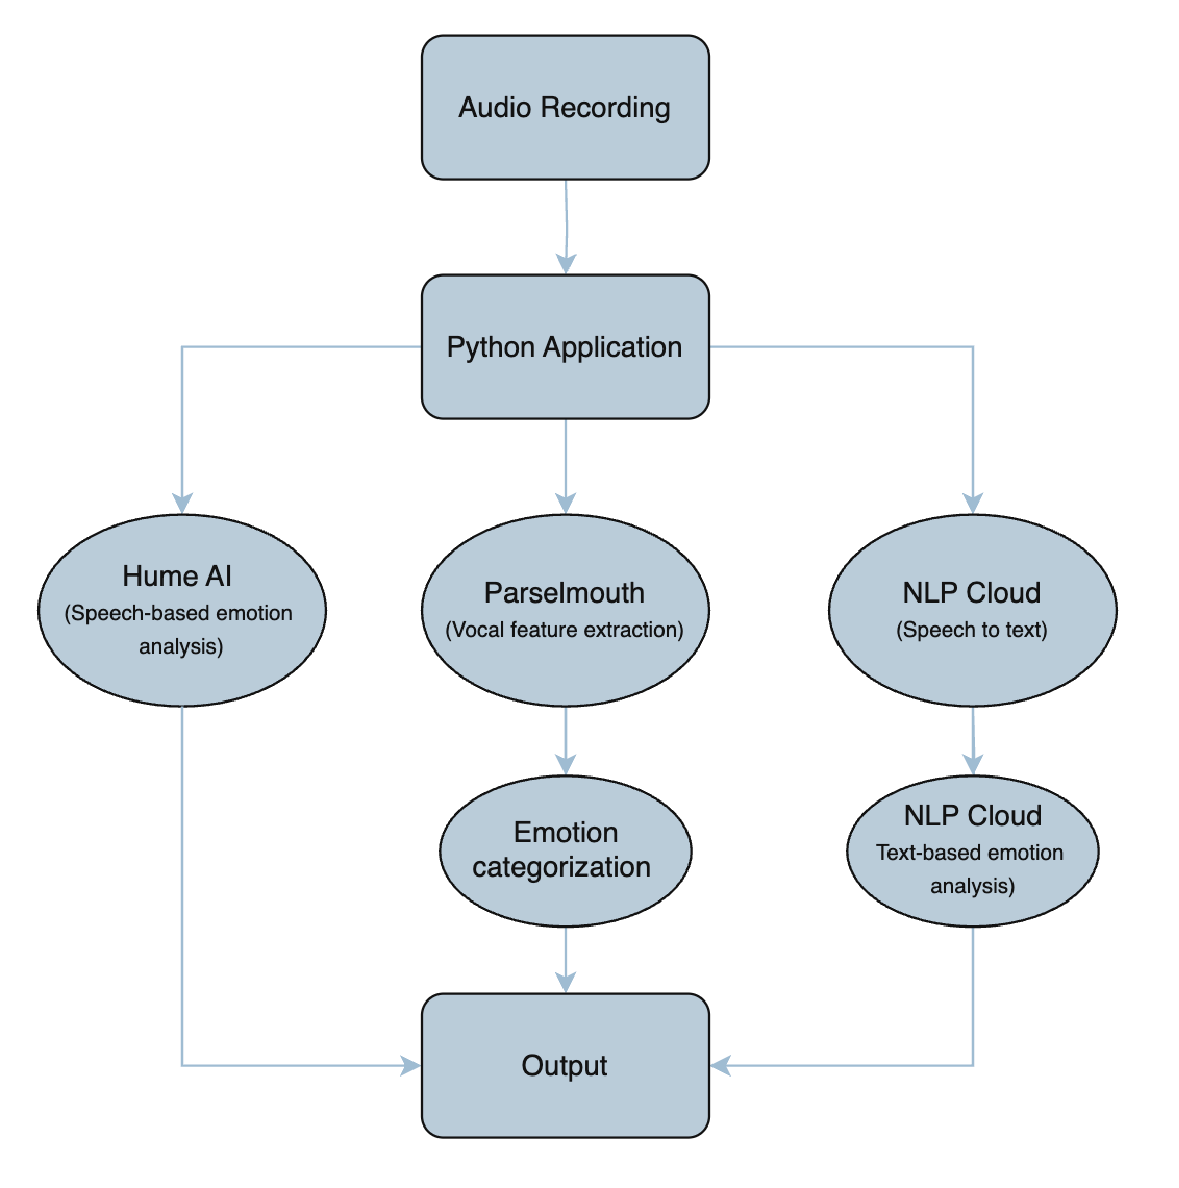
\includegraphics[width=0.6\textwidth]{png/results/rq1_nr3/python-app.pdf}
    \caption{Overview of the Python application structure.}
    \label{fig:tf-python-app}
\end{figure}
    

\subsection{Interviews and Surveys}
\label{sec:theo-interviews}

The semi-structured interviews involve voluntary participants engaging in short audio-recorded interviews, designed to draw out natural emotional responses. The participants will be asked questions to prompt them to recall and reflect on past experiences which encourages them to revisit emotions they felt at that time. 
As the format of the interviews are semi-structured and involve spontaneous speech unlike acted datasets, a well-known challenge emerges. Spontaneous vocal data tends to involve more neutral expressions, and research have shown some emotional classifiers to have a lower accuracy in detecting neutral statements \autocite{Cao2015}. This is also supported by other research, stating that acted speech shows higher levels of intensity \autocite{Chakraborty2016}. While spontaneous speech presents some documented challenges, it also reflects real word conditions.

For ethical purposes the participants will be given a selection of topics to choose from, minimizing the risk of discomfort or distress. The audio recordings will be anonymous and recorded in a controlled acoustic environment to ensure minimal noise interference.

Questions asked during the interview follow one of many emotion induction techniques, known as “autobiographical recall”. This is a method used to facilitate the re-experiencing of emotions felt in a previous moment \autocite{Siedlecka2019}, which is what is intended for the interviews to be able to collect emotional data from vocal recordings. By letting the participant think and speak about a memory from the past, emotions felt in that moment reflect in their voice.

After the interview is done, the participants will answer a survey doing a self-assessment of their emotions felt during the interview. This will enable a comparison between emotion detection and the participants reported emotional experiences.

There are many different methods for self-assessment, and emotional self-assessment is linked to many different theories. Many are connected to emotional intelligence (EI), trait emotional intelligence (trait EI) and Core Self Evaluation (CSE) \autocite{Montasem2013}, but rather than conducting a comprehensive exploration of different psychological theories in self-assessment, this research will use simplified surveys at a basic level for the purpose of fulfilling the technical objectives of the work and align with the technical focus of the thesis.

The theories behind the interviews are stated in the possibility of detecting emotions in voices. While there are a lot of recognized emotions that can be detected in different AI models and software tools, the interview will focus on bringing out two different basic emotions to maintain a manageable scope, while ensuring ethical feasibility.

Research has stated that there are different levels of unique universal signs for different affective states and while there are evidence supporting the universality for certain emotions such as anger, fear, surprise, sadness, happiness and more, there are also emotions that do not include all characteristics that distinguish them from other mental states, two examples being guilt and shame \autocite{Ekman2011}. Research of this nature supports the rationale for having the focus solely on two of the basic emotions for this thesis. The questions in the interviews will focus on bringing out two separate emotions, one on the positive spectrum, joy, and one on the negative spectrum, anger.



\section{Statistical Analysis}
\label{sec:theo-stat-analyse}

\subsubsection{Pearson Correlation Coefficient}
Pearson's r is a measurement of the strength and direction of a linear relationship between two variables. The value range is from -1 to 1, where positive values implies a positive correlation and negative values the opposite.
Values close to +-1 indicate a strong correlation, values between +-0.30 and +-0.49 a moderate correlation, and values 
below +-0.29 are seen as a weak correlation. Values around 0 implies no linear correlation \autocite{Bruce2017}.

\subsubsection{P-Value}
A p-value indicates if the observed results have a probability of occurance by chance. A widely accepted threshold for statistical significance 
is p < 0.05, which means there is less than a 5\% possibility that the observed effect is random \autocite{Bruce2017}. 

\subsubsection{Z-score Standardization}
Acoustic features such as pitch, intensity, jitter and shimmer can have great variation. To ensure comparability in statistical analyses, features are often standardized using Z-score standardization \autocite{Ekberg2023}.
This method transform data to have a mean of zero and a standard deviation of one, ensuring meaningful comparisons across features. By this, a variable does not have an overly influence due to a scale of the measurement. 
The measurements are described as "standard deviations away from the mean". \autocite{Bruce2017}. 

\subsubsection{Standardized Distance for Emotion Categorization}
Emotion categorization based on vocal features can be operated through standardized distance methods, where deviations from the baseline of acoustic profiles are quantafied. Using standardized differences allow an interpretable measure of how vocal features aligns with expected patterns for each emotion \autocite{Ekberg2023} \autocite{Bruce2017}. 
The categorization method used in this study is a custom method inspired by this standard practice. 

\subsubsection{ANOVA Tests}
ANOVA (Analysis of Variance) is a standard statistical method used to determine if there are any significant differences in means across multiple groups {Bruce2017}. It is used to categorize grouping factors and are one method in the Swedish research for vocal markers {Ekberg2023}.  

\subsubsection{Tukey's HSD}
When ANOVA presents significant differences between group means, Tukey's HSD test is incorporated as a post analysis to identify which groups are divergent from each other. 
This method controls for errors when making multiple comparisons \autocite{Bruce2017}. 
\subsubsection{T-Tests and Cohen's d}
Paired T-tests are used to compare the means between two groups to determine statistical significance, while Cohen's d provides a standardized measure of the effect size which indicates the magnitude of the observed differences \autocite{Cohen1977} \autocite{Bruce2017}.